%=============================================================================
\section{Dataset}
\label{sec:data}
%=============================================================================

\paragraph{Incidents.}
We collected 15 cross-chain DeFi incidents from 2021 to 2025 that are documented by at least one public security source (CertiK, SlowMist, Beosin, BlockSec, PeckShield, Halborn, Chainalysis or Elliptic): 8 on BSC, 5 on Arbitrum and 2 on Ethereum (Appendix~\ref{app:incidents}).
The 82-case list of AMLGuard~\cite{wu2026amlguard} was used only to locate candidates; every seed address, start block and exit was verified on-chain by the authors against the public report.
For 10 incidents the report confirms the exit (bridge, mixer or lending deposit) and the endpoint is defined as in Sect.~\ref{sec:problem}; the other 5 are used for detection but not for lead time.

\paragraph{Hard negatives.}
A detector that separates stolen funds from dormant wallets is useless in practice, because an analyst watching a bridge sees mostly legitimate users.
We therefore mine negatives from the \emph{same} protocols and time window as each incident.
For each incident we list the verified bridge, DEX and mixer contracts on its trace and collect every counterparty of these contracts within $\pm7$ days.
A candidate is accepted if it interacted directly with the contract, received or sent a positive value, did not fan out to more than three addresses (split-like pattern), and made no mixer deposit after a non-mixer interaction.
Seeds of all incidents and the 82 AMLGuard addresses are excluded.
A second pass targets complex benign activity: it requires at least $\mathrm{e}^{0.35\log(1+n^+)}-1$ raw events, where $n^+$ is the length of the incident trajectory, and relaxes the fan-out bound on a log scale for incidents with a large fan-out.
Five manually selected controls, one per early incident (for example, a legitimate Ronin withdrawal followed by a swap in the same hour), complete the set.
Each negative is expanded with exactly the same collector, builder and depth as the incidents.

\paragraph{Collection and completeness.}
We re-collected all raw data for this paper through the free tiers of Etherscan (Ethereum, Arbitrum) and NodeReal (BSC): \TBD{1.5}\,GB of responses over \TBD{N} API calls.
A trajectory enters the dataset only if every address it reaches has a complete cache.
The monthly NodeReal quota ran out before all BSC negatives were collected, so 223 of the 272 BSC negatives in the mining registry are excluded, and for one BSC incident (Paraluni) the trajectory is rebuilt from our earlier decoded trace of the same seed and window, truncated to the same depth.
No transaction appears in two incident groups; a few infrastructure addresses (routers, pools, exchange wallets) are shared, which cannot leak labels because no feature encodes address identity.

\paragraph{Statistics.}
Table~\ref{tab:data} summarizes the dataset and Fig.~\ref{fig:data} contrasts incidents with negatives.
Incident trajectories are longer (median \TBD{40} vs.\ \TBD{3} actions) and richer in swaps and bridge deposits; because raw action counts and prefix length are not model inputs and checkpoints are evaluated separately, length alone cannot explain the results (Sect.~\ref{sec:results}).

\begin{table}[t]
\centering
\caption{Real-data statistics. Prefix rows are extracted at $k\in\{2,3,5,7\}$ and at 25/50/75/100\% of each trajectory; duplicates of the same (trajectory, $k$) are pooled once.}
\label{tab:data}
\small
\begin{tabular}{@{}lrrrr@{}}
\toprule
 & Ethereum & BSC & Arbitrum & Total \\
\midrule
Incidents & 2 & 8 & 5 & 15 \\
Hard negatives & \TBD{} & \TBD{} & \TBD{} & \TBD{393} \\
Actions & \TBD{} & \TBD{} & \TBD{} & \TBD{11{,}721} \\
Prefix rows (pooled, deduplicated) & & & & \TBD{1{,}384} \\
Positive rate of pooled rows & & & & \TBD{8.4\%} \\
\bottomrule
\end{tabular}
\end{table}

\begin{figure}[t]
\centering
\begin{subfigure}[t]{0.49\linewidth}\centering
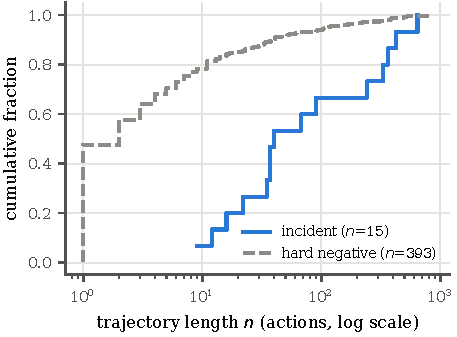
\includegraphics[width=\linewidth]{figures/fig2a.pdf}
\caption{Trajectory length (ECDF).}
\label{fig:2a}
\end{subfigure}\hfill
\begin{subfigure}[t]{0.49\linewidth}\centering
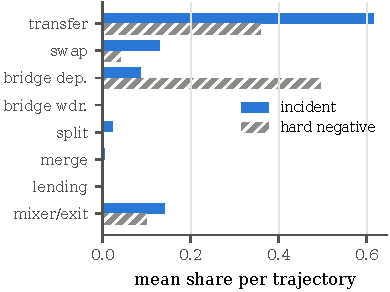
\includegraphics[width=\linewidth]{figures/fig2b.pdf}
\caption{Mean share of each action type.}
\label{fig:2b}
\end{subfigure}
\caption{Incidents versus hard negatives in the real dataset.}
\label{fig:data}
\end{figure}

\paragraph{Synthetic benchmark (CAGI-Synth).}
Fifteen incidents limit statistical power, and the real negatives cannot be made harder on demand.
We therefore also release a \emph{synthetic} benchmark, reported separately from every real-data result.
Its generator samples laundering trajectories from five typologies taken from public reports and AADAPT (peel chain to a bridge; split, swap to a stablecoin and bridge; swap and fixed-denomination mixer deposits; nested bridges; lending round trip), and benign trajectories from six ordinary behaviours (bridge user, DEX trader, payroll split, consolidation, arbitrage bot, single mixer deposit) padded with routine activity so that lengths overlap.
A difficulty knob $d\in[0,1]$ controls two things: with probability $d$ a benign trajectory is drawn from laundering-like behaviours (bridge, swap and split within minutes; hop through fresh wallets to a bridge; fast rotation of funds), and with probability $d$ per step the launderer inserts small decoy transfers and slows down.
We generate 30 synthetic incidents with 40 negatives each at $d\in\{0,0.25,0.5,0.75,1\}$.
